\sloppy
\documentclass[14pt,a4paper,oneside]{extarticle}	% Размер основного шрифта и формата листа
\usepackage{xltxtra}						% Используется для вывода логотипа XeLaTeX
\usepackage{xunicode}						% Кодировка документа
\usepackage{polyglossia}					% Загружает пакет многоязыковой верстки
\newfontfamily\russianfont{Book Antiqua}
%\setmainfont{Liberation Serif}						% Основной шрифт текста
\setmainfont{Book Antiqua}
\setdefaultlanguage{russian}				% Основной язык текста
\setotherlanguage{english}					% Дополнительный язык текста
\linespread{1}							% Межстрочный интервал выбран полуторным
\usepackage[left=2.5cm,
right=1.5cm,vmargin=2.5cm]{geometry} % Отступы по краям листа
\bibliographystyle{ugost2008}

\usepackage{xcolor}
\usepackage{hyperref}
% Цвета для гиперссылок
\definecolor{linkcolor}{HTML}{359B08} % цвет ссылок
\definecolor{urlcolor}{HTML}{799B03} % цвет гиперссылок
\hypersetup{pdfstartview=FitH,  linkcolor=linkcolor,urlcolor=urlcolor, colorlinks=true}

%---------------------------%
%---- Пакеты расширений ----%
%---------------------------%
\usepackage{xcolor}
\usepackage{hyperref}
% Цвета для гиперссылок
\definecolor{linkcolor}{HTML}{359B08} % цвет ссылок
\definecolor{urlcolor}{HTML}{799B03} % цвет гиперссылок
\hypersetup{pdfstartview=FitH,  linkcolor=linkcolor,urlcolor=urlcolor, colorlinks=true}


\usepackage{verbatim,indentfirst}
\usepackage{cite,enumerate,float}
\usepackage{amsmath,amssymb,amsthm,amsfonts}

%---------------------------%
%--- Вставка иллюстраций ---%
%---------------------------%
\usepackage{graphicx}
\usepackage{subfigure}
%\graphicspath{{Images/}}
\usepackage{fontspec}

\begin{document}
%	\pagestyle{empty} %  выключаенм нумерацию
	
	%\setcounter{page}{3}% Нумерация начинается с третьей страницы
	%\renewcommand{\contentsname}{\center{Содержание}}
	%\tableofcontents
	
	\newpage
	\begin{center}
		%\addcontentsline{toc}{section}{Маятник Максвелла}
		\subsection*{Маятник Максвелла}
	\end{center}

\begin{figure}[H] 	
	\centering 	
	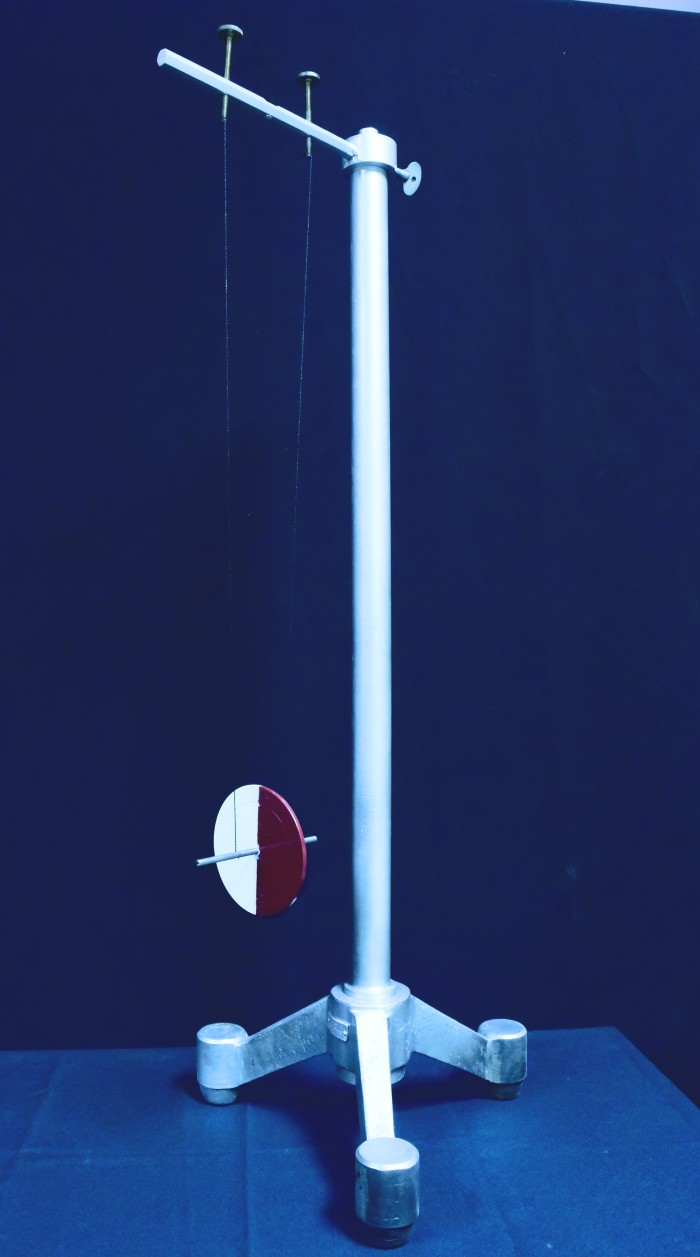
\includegraphics[width=0.5\linewidth]{Maxwell-1.png}
	\caption{Демонстрация перехода потенциальной энергии в кинетическую и обратно}
	\label{Maxwell-1}
\end{figure}

\subsection*{\underline{Оборудование:}}
\begin{enumerate}
	\item Металлический диск радиусом 5 см и массой 500 г на бифилярном подвесе.
	\item Штатив с металлическим стержнем.
\end{enumerate}
	
\newpage
\subsection*{\underline{Основные определения:}}
		
Можно показать, что если тело вращается относительно оси, проходящей через его центр масс, и одновременно перемещается поступательно так, что ось смещается параллельно самой себе, то согласно теореме Кёнига
\begin{flushleft}
\textit{полная кинетическая энергия твердого тела равна сумме кинетической энергии поступательного движения центра масс тела (считая сосредоточенной в нем массу тела) и кинетической энергии вращения тела:}
\end{flushleft}
$$ E_\text{к} = \frac{mv_c^2}{2} + \frac{I\omega^2}{2}, $$
где $ v_c $ — скорость поступательного движения центра масс, \textit{I} — момент инерции тела относительно оси вращения, проходящей через центр масс, $ \omega $ — угловая скорость вращения тела вокруг той же оси.

Следует также отметить, что энергия вращательного движения при заданной угловой скорости существенно зависит от распределения в теле массы – момента инерции.
Отсюда становится понятным, зачем маховики делают с большим моментом инерции.
Очевидно, чтобы увеличить при данной угловой скорости его кинетическую энергию.
Значительный запас энергии кинетический энергии необходим, например, для сохранения равномерности хода двигателя механизма при внезапно меняющейся нагрузке.
	
\newpage
\subsection*{\underline{Краткое описание:}}


Для демонстрации законов сохранения применяется маятник Максвелла, представляющий собой массивный диск радиусом \textit{R} и массой \textit{m}, туго насаженный на ось радиусом \textit{r}, за которую маятник подвешивается на двух нитях к металлическому стержню (рис.\ref{Maxwell-1}).

Для выполнения демонстрации стержень укрепляется на физическом штативе.
Поворачивая концы оси обеими руками, накручивают на нее нити так, чтобы витки укладывались в один ряд и навинчивались от концов оси к диску (!!!).
При этом диск поднимается на некоторую высоту.

Затем отпускают ось.
Диск, вращаясь, начинает опускаться вниз и разматывает нити.
В крайнем нижнем положении скорость вращения диска будет наибольшей.
Далее лиск, вращаясь по инерции, наматывает нить на ось и поднимается вверх (рис.\ref{Maxwell-2}).
Теперь скорость вращения диска будет постепенно уменьшаться, пока он не остановится почти на той же высоте, с которой его пустили.
После этого диск, вращаясь, снова начнет опускаться вниз, а потом подниматься вверх и т.д.

Подъем и опускание диска будут продолжаться до тех пор, пока запас энергии, который сообщили диску при его подъеме на некоторую высоту, не израсходуется на преодоление упругости нити, на трение оси с нитью и на сопротивление воздуха.

Таким образом, сущность демонстрации заключается в следующем: если данной системе, состоящей из массивного диска на оси, сообщить некоторое количество энергии (совершить работу, подняв диск на определенную высоту), то последняя почти целиком (за исключением потерь) переходит из одной формы в другую.
В данном случае энергия потенциальная (энергия положения) переходит в энергию кинетическую (энергию вдижения) и наоборот.

Если во время опускания диска несколько нажать на ось вниз, то диск начнет вращаться быстрее и поднимется затем выше уровня, с которого его пустили.
Дополнительное количество энергии, которое при этом сообщили системе, прибавится к имеющемуся запасу и будет влиять на максимальную скорость вращения и высоту подъема диска.
	
\begin{figure}[H] 	
\centering 	
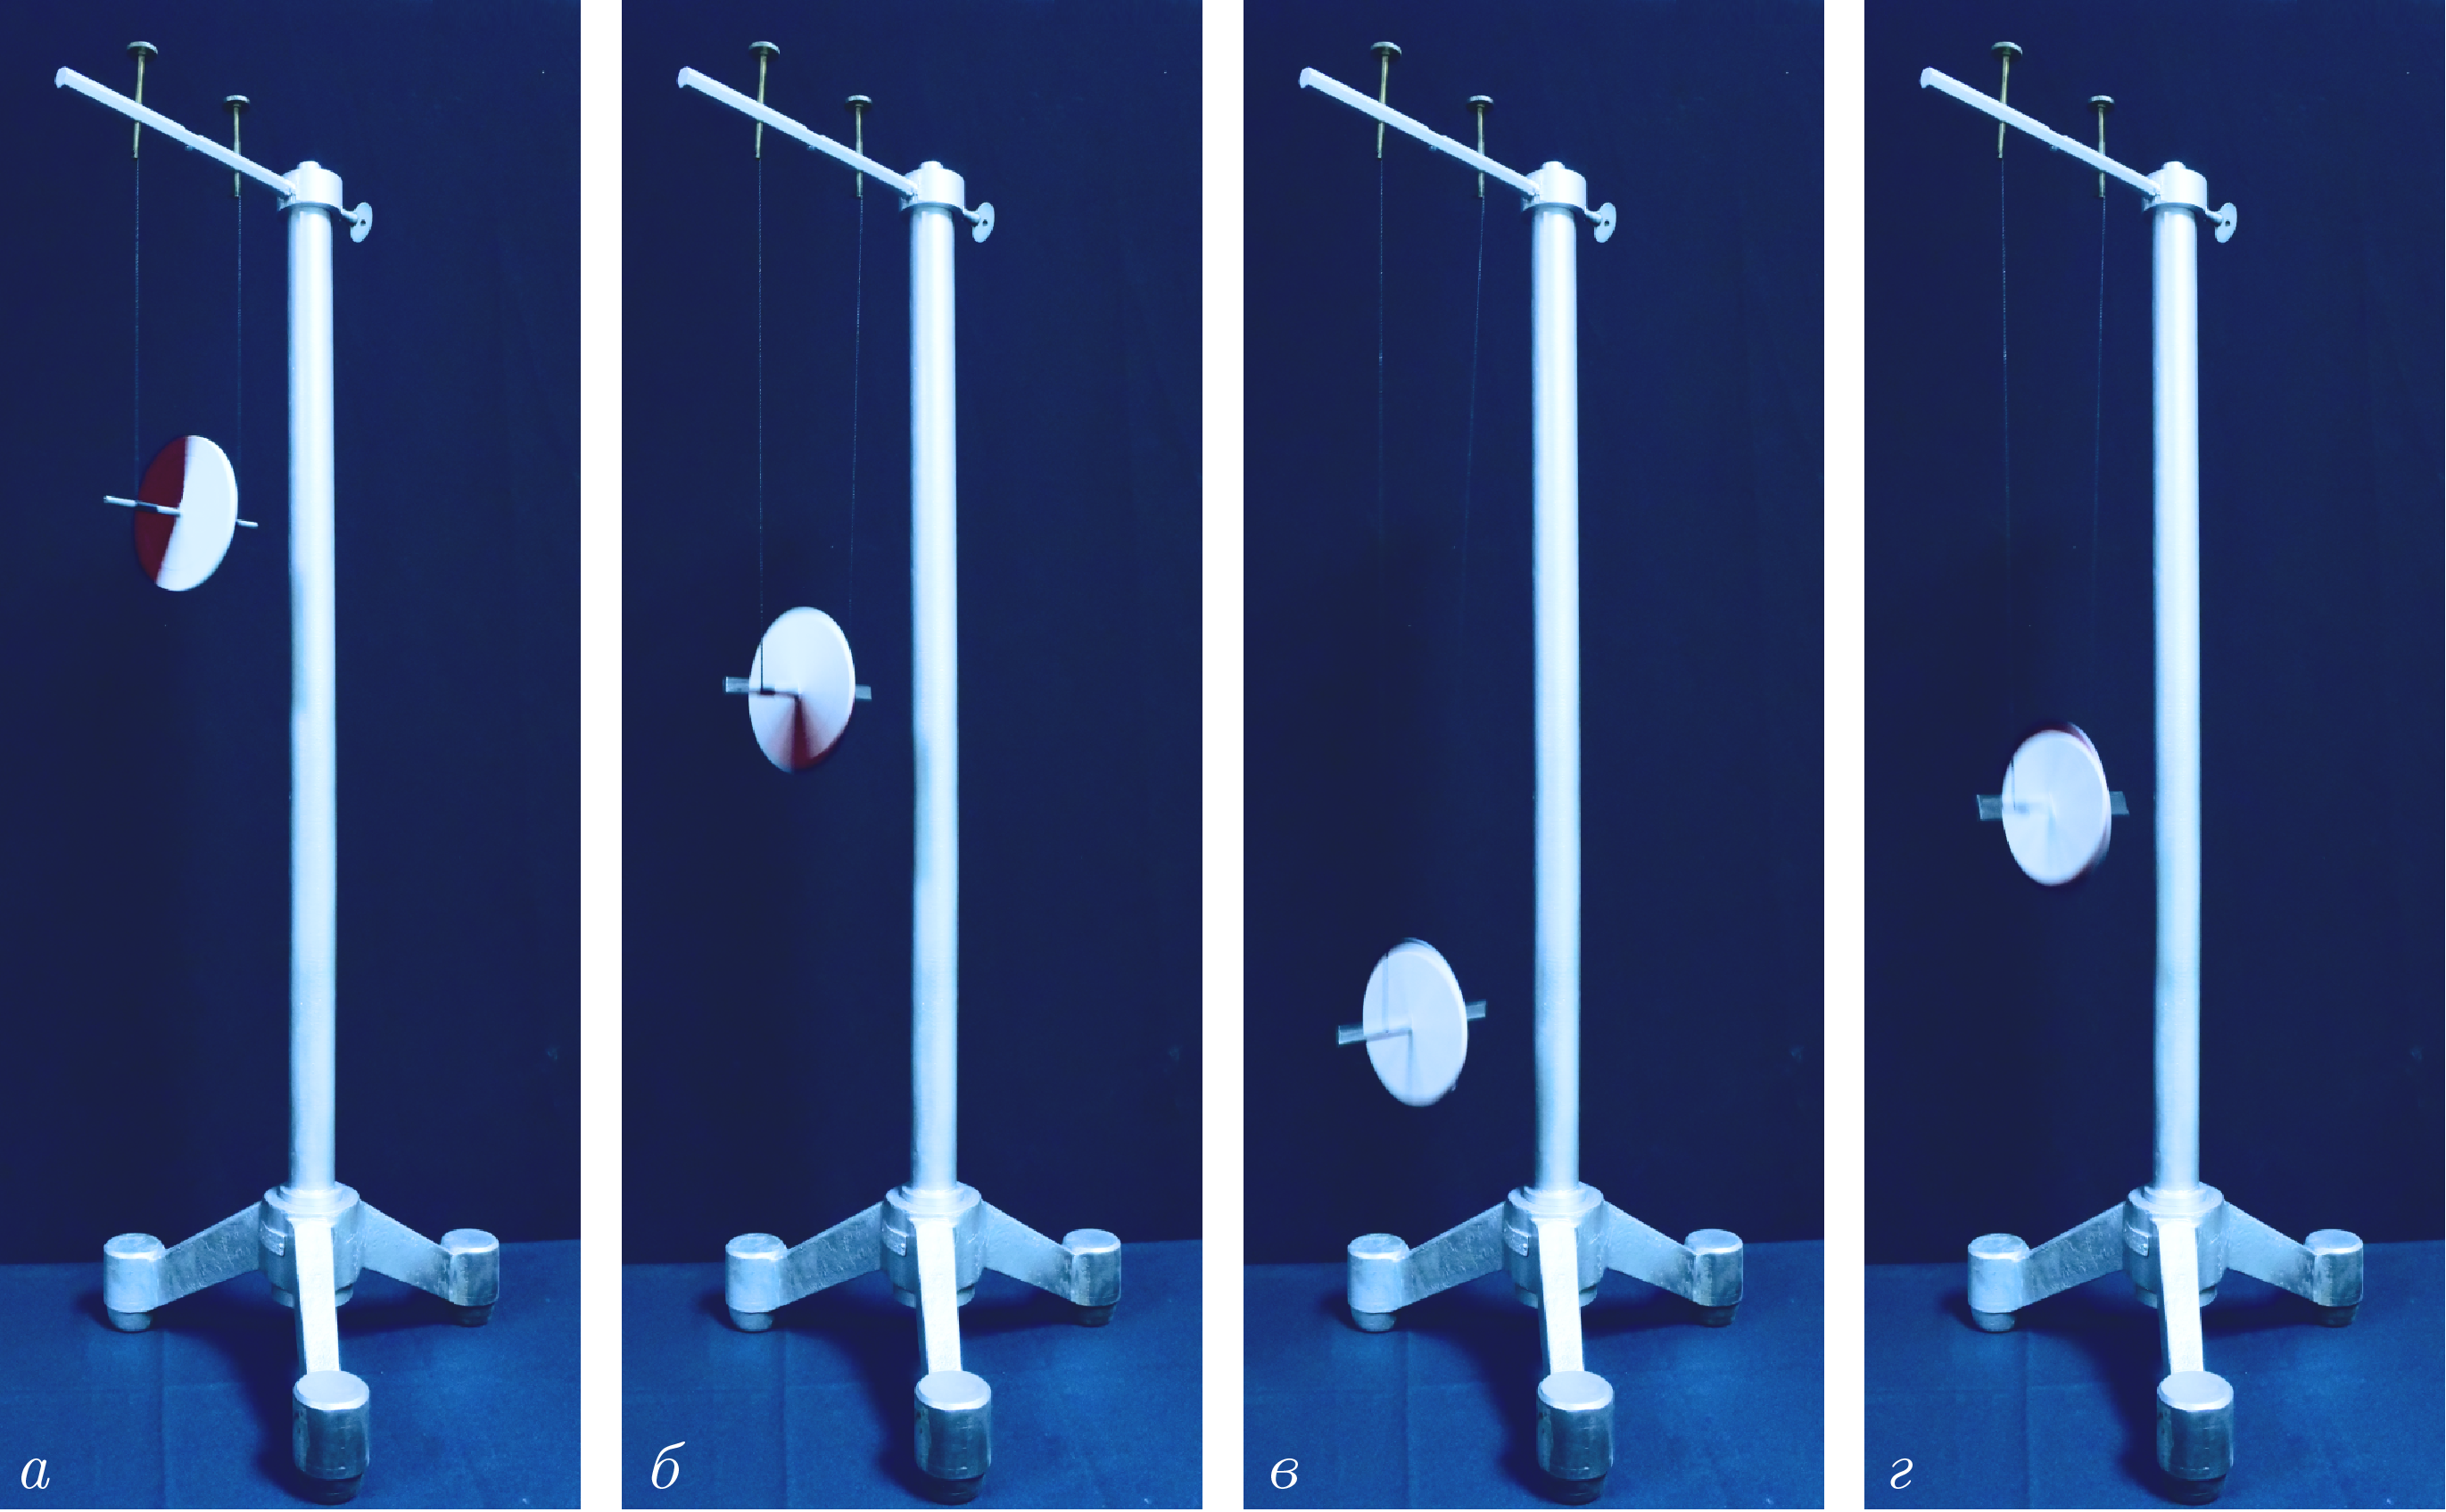
\includegraphics[width=0.9\linewidth]{Maxwell-2.png}
\caption{Фотографии различных состояний маятника Максвелла: \textit{а} — начальное положение с наибольшей потенциальной энергией; \textit{б} — подвес маятника раскрутился наполовину; \textit{в} — диск маятника находится в самой нижней точке и обладает наибольшей кинетической энергией}
\label{Maxwell-2}
\end{figure}
	
\textit{Подготовка опыта}: При подготовке демонстрации надо обратить внимание на следующее:

а) Стержень следует установить в штативе горизонтально и достаточно прочно зажать в муфте винтом.

б) Штатив рекомендуется использовать наиболее массивный, чтобы устранить колебания всей системы.

в) Ось вращения диска должна быть расположена горизонтально.

г) Нити нужно брать одинаковой длины и симметрично расположить их относительно диска; расстояние между нитями у стержня должно быть несколько меньше, чем у оси.
	
\newpage
\subsection*{\underline{Теория:}}
		
	 Когда маятник отпускается, он совершает возвратно-поступательное движение в вертикальной плоскости при одновременном вращении диска вокруг оси.
	
		\begin{figure}[H] 	
		\centering 	
		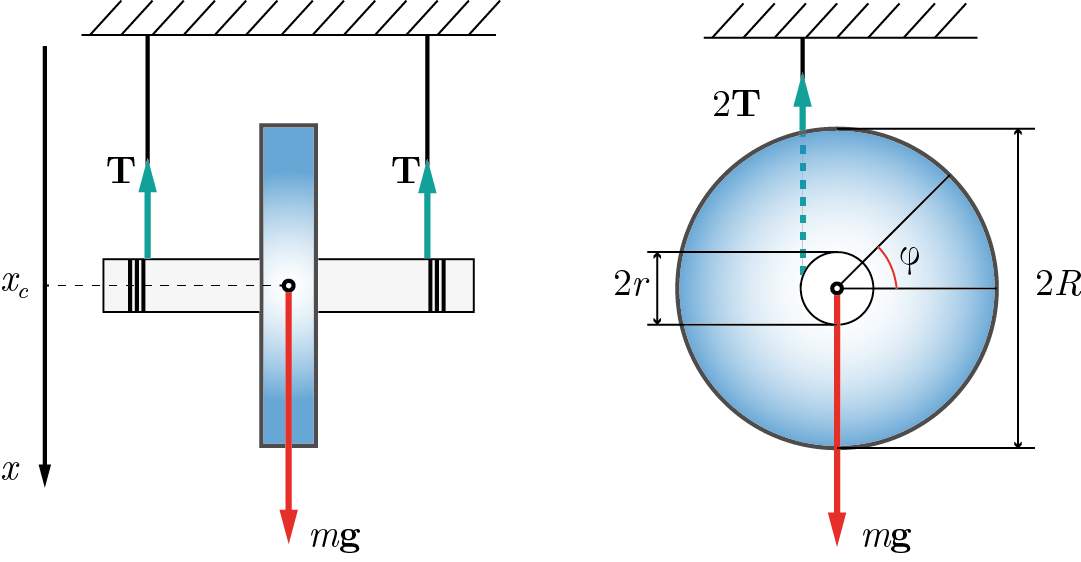
\includegraphics[width=0.9\linewidth]{Maxwell-3.png}
		\caption{Схематичное изображение сил, действующих на массивный диск в маятнике Максвелла}
		\label{Maxwell-3}
	\end{figure}
	 
	Измеряя расстояние, пройденное диском, и время движения можно рассчитать момент инерции маятника Максвелла.
	На рис.\ref{Maxwell-3} указаны силы, действующие на маятник.
	Для описания движения маятника удобно выбрать систему отсчета, связанную с центром масс маятника.
	Центр масс маятника опускается вниз с линейным ускорением \textbf{a}.
	Уравнение движения центра масс маятника имеет вид:
	\begin{equation}\label{Maxwell-1eq1}
	m\textbf{a} = m\textbf{g} + \textbf{T},
	\end{equation}
	где \textbf{T}  — сила натяжения каждой из нитей, $ m $ — масса маятника.
	
	Необходимо учесть, что маятник совершает также вращательное движение вокруг горизонтальной оси, проходящей через центр масс под действием момента силы натяжения нитей $ M = r T $, где $ M $ – момент сил натяжения $ T $, а $ r $ — радиус вала.
	
	Основное уравнение вращательного движения имеет вид
	\begin{equation}\label{Maxwell-1eq2}
	\textbf{M} = I\textbf{ε},
	\end{equation}
	где \textbf{ε} — угловое ускорение вращения маятника, $ I $ — момент инерции маятника.
	
	Спроектируем силы на направление движения маятника.  
	Так как центр масс маятника опускается на столько, на сколько раскручивается нить, то перемещение $ x $ центра масс связано с углом поворота $ \varphi $ соотношением:
	\begin{equation}\label{Maxwell-1eq3}
	x = \varphi r
	\end{equation}
	Дифференцируя это выражение дважды по времени, получим
	\begin{equation}\label{Maxwell-1eq4}
	a = \frac{d^{2} x}{d t^{2}} = r\frac{d^{2} \varphi}{d t^{2}} = r \varepsilon.
	\end{equation}
	
	С учетом выражения (\ref{Maxwell-1eq2}) уравнение (\ref{Maxwell-1eq4}) можно переписать следующим образом 
	\begin{equation}\label{Maxwell-1eq5}
	rT = \frac{Ia}{r}.
	\end{equation}
	
	Приведем полученное выражение к виду
	\begin{equation}\label{Maxwell-1eq6}
	T = \frac{Ia}{r^{2}}.
	\end{equation}
	
	Учитывая уравнение (\ref{Maxwell-1eq1}), получим выражение для линейного ускорения центра масс маятника
	\begin{equation}\label{Maxwell-1eq7}
	a = \frac{mg}{m + \frac{I}{r^{2}}},
	\end{equation}
	а для силы натяжения нити:
	
	\begin{equation}\label{Maxwell-1eq8}
	T = \frac{mg}{1 + mr^2/I}
	\end{equation}
	
	Из полученных соотношений следует, что ускорение маятника и сила натяжения нити не изменяются со временем. 
	Следовательно, если при опускании маятника координату $ x_c $ его центра масс отсчитывать от начального положения равновесия, ось направить вниз, то со временем положение маятника меняется по закону:
	
	\begin{equation}\label{Maxwell-1eq9}
	x_c = \frac{at^{2}}{2}
	\end{equation}
	
	Подставляя выражение (\ref{Maxwell-1eq8}) в уравнение (\ref{Maxwell-1eq9}), получим для момента инерции маятника Максвелла следующее выражение
	\begin{equation}\label{Maxwell-1eq10}
	I = mr^{2}\left(\frac{gt^{2}}{2h} - 1 \right),
	\end{equation}
	в которое входят измеримые в эксперименте величины, такие как $ r $ — радиус вала с намотанной на него нитью, $ h $ — координата центра масс в нижней точке траектории (начальная высота), $ m $ — масса маятника.
	Необходимо учитывать, что масса маятника Максвелла складывается из массы вала и диска.
	
	
\end{document}
